\documentclass{article}
\usepackage[utf8]{inputenc}
\usepackage{amsmath}
\usepackage{geometry}
\usepackage{graphicx}
\usepackage[T1]{fontenc}
\usepackage{fourier}
\usepackage{float}
\usepackage{subfig}

\title{BIM3007-Assignment4}
\author{Junyang Deng}
\date{\today}
\geometry{left=3cm,right=3cm,top=2cm,bottom=2cm}
\setlength{\parindent}{0cm}
\linespread{1.3}
\begin{document} 
\maketitle
\section{RNA-Seq}
\begin{enumerate}
    \item In RNA-seq analysis, what is the significance of data quality control? What softwares can be used for quality control? \emph{(10 points)}
    
    \textbf{Significance}: Quality control is usually the first step in any RNA-seq analysis because it helps ensure the reliability of downstream analysis. Specifically, quality control can improve the accuracy of alignment and make differential analysis or functional annotation more reliable.

    \textbf{Softwares} for quality control include FastQC, RSeQC, MultiQC, RNASeqQC etc. In tutorial we learned about \textbf{FastQC} and \textbf{MultiQC}.
    
    \begin{itemize}
        \item FastQC: When a \texttt{.fastq} file is input, this software will generate a report for the data in \texttt{.html} format. The report includes the following tests and results (Figure~\ref{fig:fastqc}). The mark in front of each item indicates the test result. A green tick means `pass', an exclamation mark means `warning', and a red cross means `failure'.
    \begin{figure}[htbp]
        \centering
        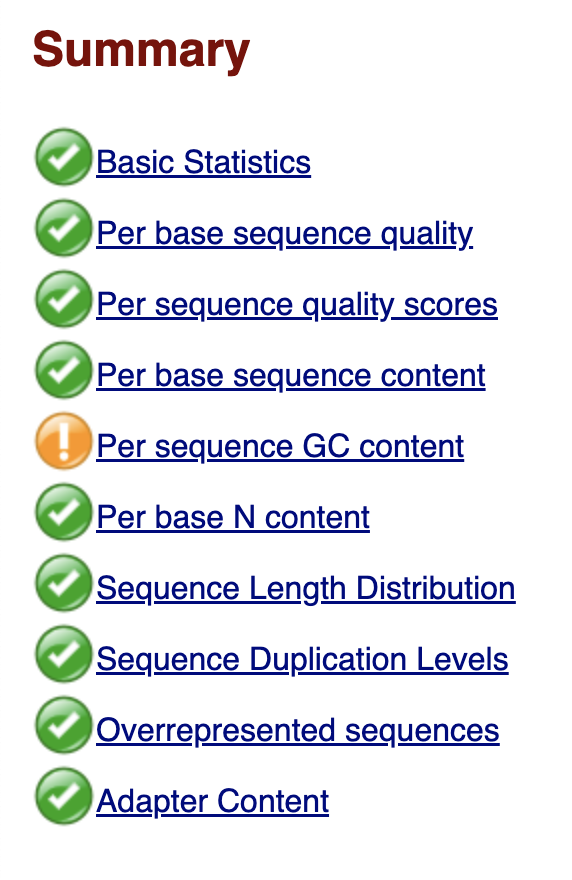
\includegraphics[width=0.3\linewidth]{images/fastqc.png}
        \caption{Fastqc report}
        \label{fig:fastqc}
    \end{figure}
    \item MultiQC: This software can be used to combine the results from multiple QC tools into a single report. It allows you to easily compare the results from different samples or different analysis pipelines.
\end{itemize}

    \item After performing the data quality control for the RNA-Seq reads, we need to align the reads to the reference genome. What is the alignment program and what is the purpose of the alignment? \emph{(10 points)}
    
    \textbf{Significance}: Alignment helps people identify the corresponding gene of the transcript. With alignment information, people can use RNA-seq data to quantify the expression level of each gene or identify alternative splicing. 
    
    \textbf{Softwares} for alignment can be divided into two types: Splice-aware aligners (STAR, TopHat, HiSat) and non-splice aligners (BWA, Bowtie and HiSat). 
    \textbf{Splice-aware aligners} are willing to open gaps rather than mismatches when two sequences cannot coincide. On the contrary, \textbf{non-splice-aware aligners} are more likely to generate mismatches, and gaps usually have higher penalties. The splice-aware ones can be used when transcripts are mapped to the whole genome, while the non splice-aware ones can be used to map 

    \item After alignment step, we obtain bam files. What program help us to summarize the gene counts? \emph{(10 points)}
    
    Program: featureCounts. This program will generate a table of genes by samples with raw sequence abundances.
    \begin{figure}[htbp]
        \centering
        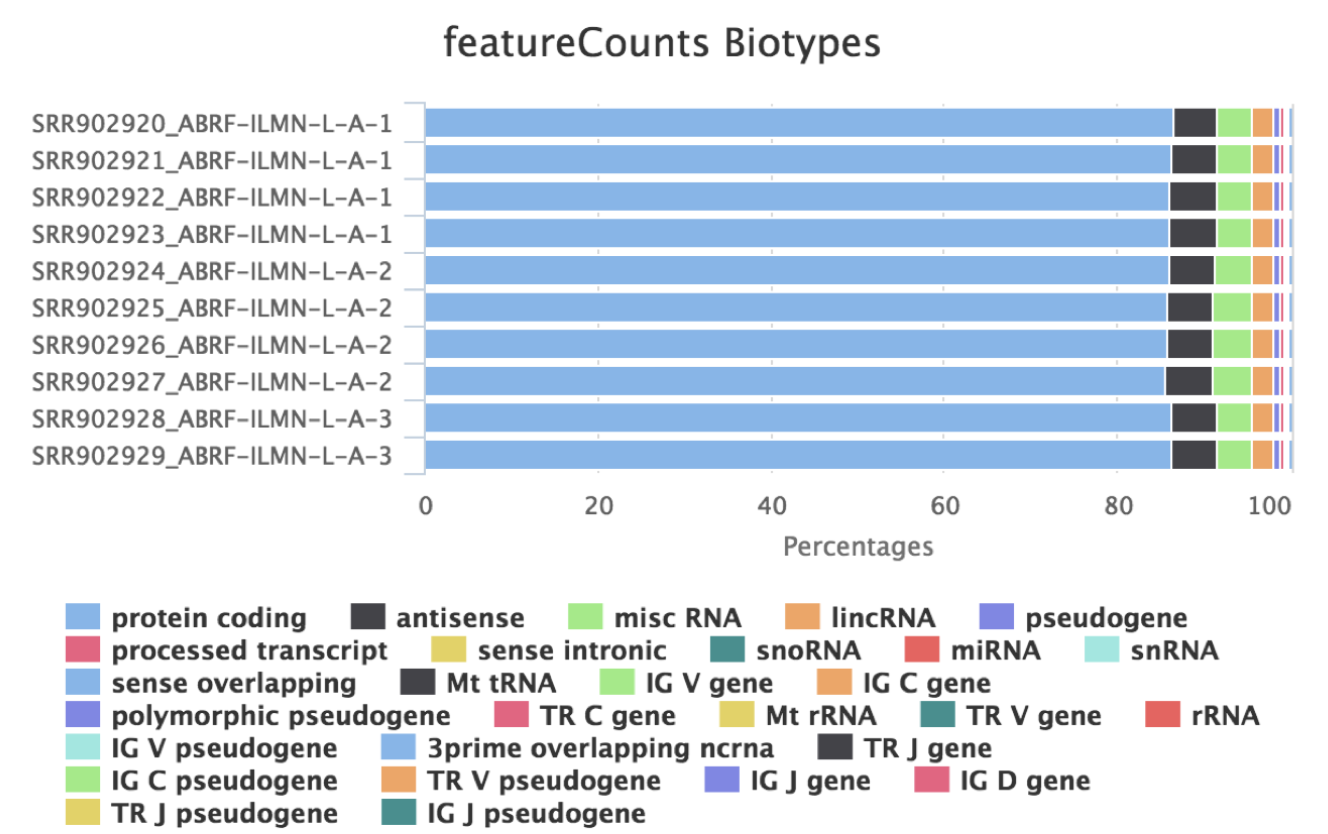
\includegraphics[width=0.8\linewidth]{images/feature-count.png}
        \caption{An example of table generated by featureCounts.}
        \label{fig:feature}
    \end{figure}

    \item What is the input and output of the standard RNA-seq analysis (featureCounts program analysis as the end point), and what kind of analysis can we do on its output? \emph{(10 points)}
    
    Input: \texttt{.fastq} file\\
    Output: a read count matrix\\
    Analysis: Many R packages can be used to conduct downstream analysis. For differential expressed gene (DEG) analysis can be done using DESeq2, limma and edgeR. After finding DEGs, we can do functional analysis using EnrichR and GSEA.

\end{enumerate}

\section{PTM Prediction Preprocessing}
\begin{enumerate}
    \item Please write a python script to extract the positive dataset and the negative dataset (13-mer) from the raw dataset (\texttt{Ubiquitination\_sites.txt}), and use CD-HIT program with cut-off values of sequence similarity of 80\% to remove the homologous sequences of both datasets. Please provide a table for the data statistics of positive and negative sequences before and after removing the homologous sequences. (30 points)
    
    The Python script used to extract the (13-mer) positive and negative dataset is named \texttt{processing.py}. The program did the following things:
    \begin{enumerate}
        \item For a site in a protein sequence, a sequence fragment with $2n + 1$ amino acids
        is constructed by taking $n$ upstream residues and n downstream residues from the site, respectively. The $n$ here is $6$;
        \item When the residues are not enough, e.g. for the sites located in N- or C-terminus,
        assign a non-existing residue X to fill in the corresponding position;
        \item Delete the negative sequences where a real ubiquitination site is involved.
    \end{enumerate}
    \begin{figure}[htbp]
        \centering
        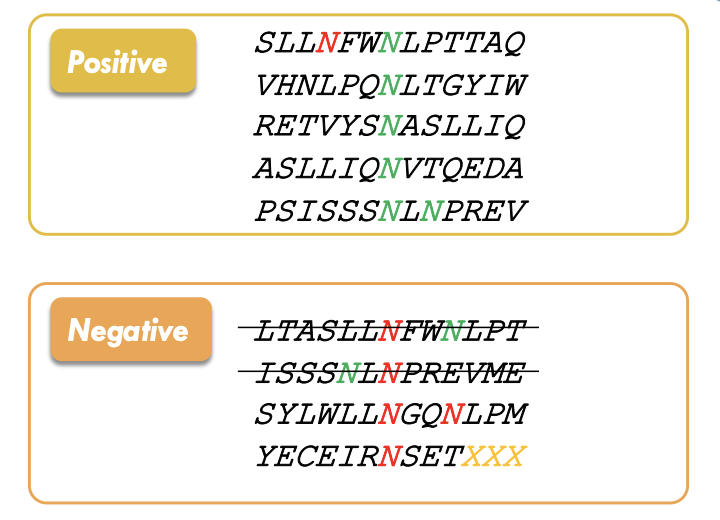
\includegraphics[width=0.7\linewidth]{images/illustration.png}
        \caption{An illustration of what the program does}
        \label{fig:illustrate}
    \end{figure}
    These steps are illustrated by Figure~\ref{fig:illustrate}. After running the script, \texttt{positive.fasta} and \texttt{negative.fasta} were generated since \texttt{.fasta} file is needed for CD-HIT. Names for sequences are just numbers. The output of CD-HIT is \texttt{positive\_80.fasta} and \texttt{negative\_80.fasta}. Statistics before and after removing homologous sequences is shown in Table~\ref{tab:statistics}. 

    \begin{table}[htbp]
        \centering\begin{tabular}{lll}
            \hline
            & Positive & Negative \\ \hline
     Before & 8,000    & 39,291   \\
     After  & 7,429    & 32,141   \\ \hline
     \end{tabular}
        \caption{Data statistics before and after removing homologous sequences}
        \label{tab:statistics}
    \end{table}

    \item After the removal of homologous sequences, please apply WebLogo tool to generate sequence logos for positive sequences and negative sequences, respectively. Then, please employ TwoSampleLogo tool to conduct the comparison of position-specific AAC between positive and negative data. (15 points)
    
    \textbf{One sample logo}: The logo of positive and negative sequences are shown in Figure~\ref{fig:pos-logo} and \ref{fig:neg-logo}. Two plots look identical with K standing in the middle. Since only K is visible in this plot, and no information is shown here, two zoomed logo plots are also given in Figure~\ref{fig:pos-zoom} and \ref{fig:neg-zoom}. Now, more information is shown. Besides logo plot, probability plots are shown in Figure~\ref{fig:pos-prob} and \ref{fig:neg-prob}. 
    
    \begin{figure}[htbp]
        \parbox{0.5\linewidth}{
            \centering
            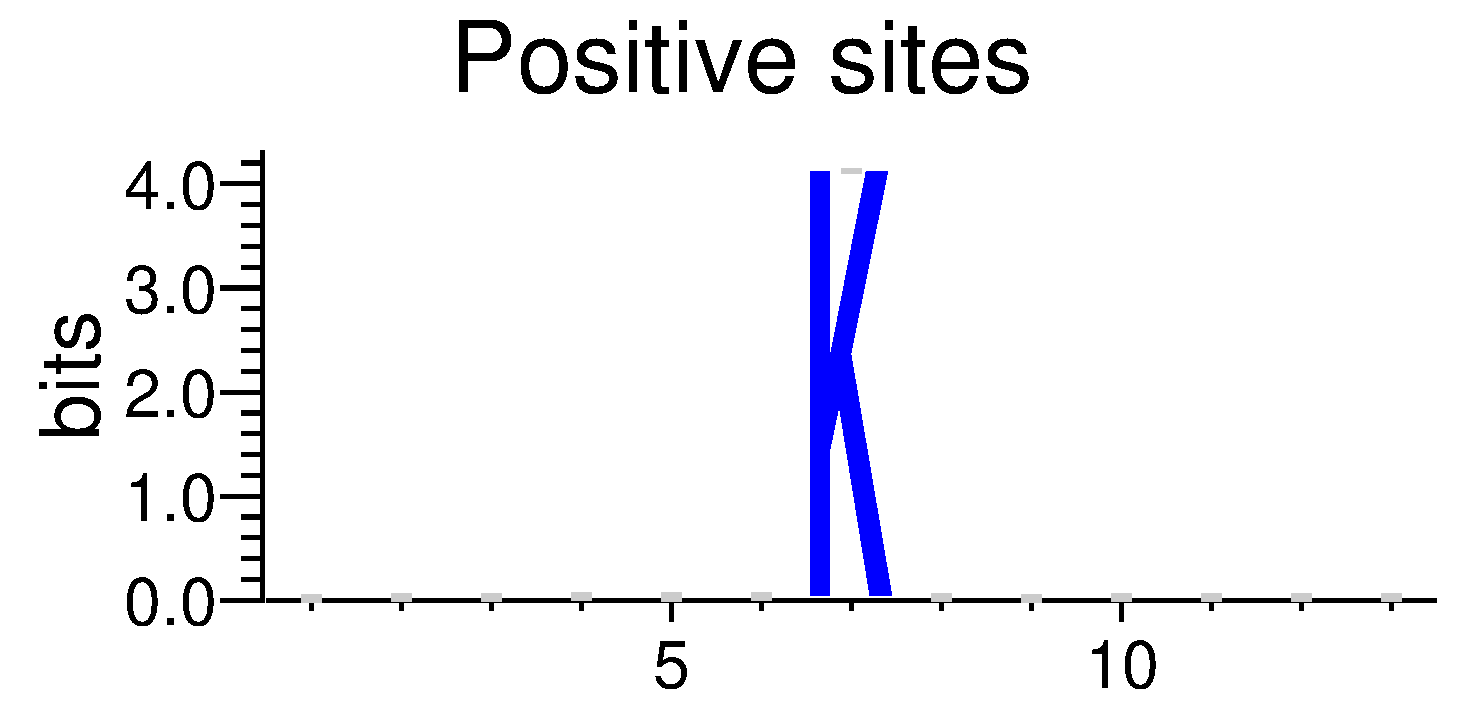
\includegraphics[width=\linewidth]{images/positive_logo.png}
            \caption{Logo of positive sequences}
            \label{fig:pos-logo}
        }
        \hfill
        \parbox{0.5\linewidth}{
            \centering
            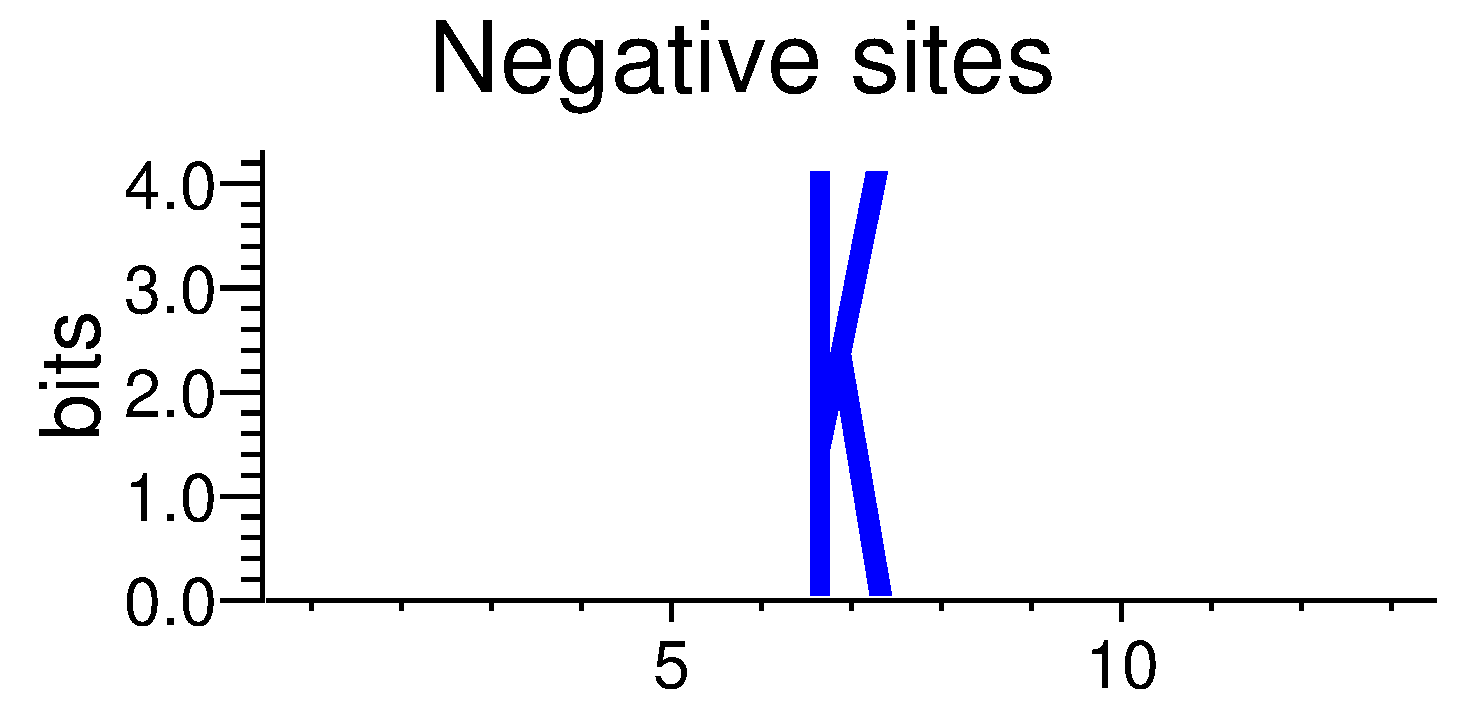
\includegraphics[width=\linewidth]{images/negative_logo.png}
            \caption{Logo of negative sequences}
            \label{fig:neg-logo}
        }
    \end{figure}
    \begin{figure}[htbp]
        \parbox{0.5\linewidth}{
            \centering
            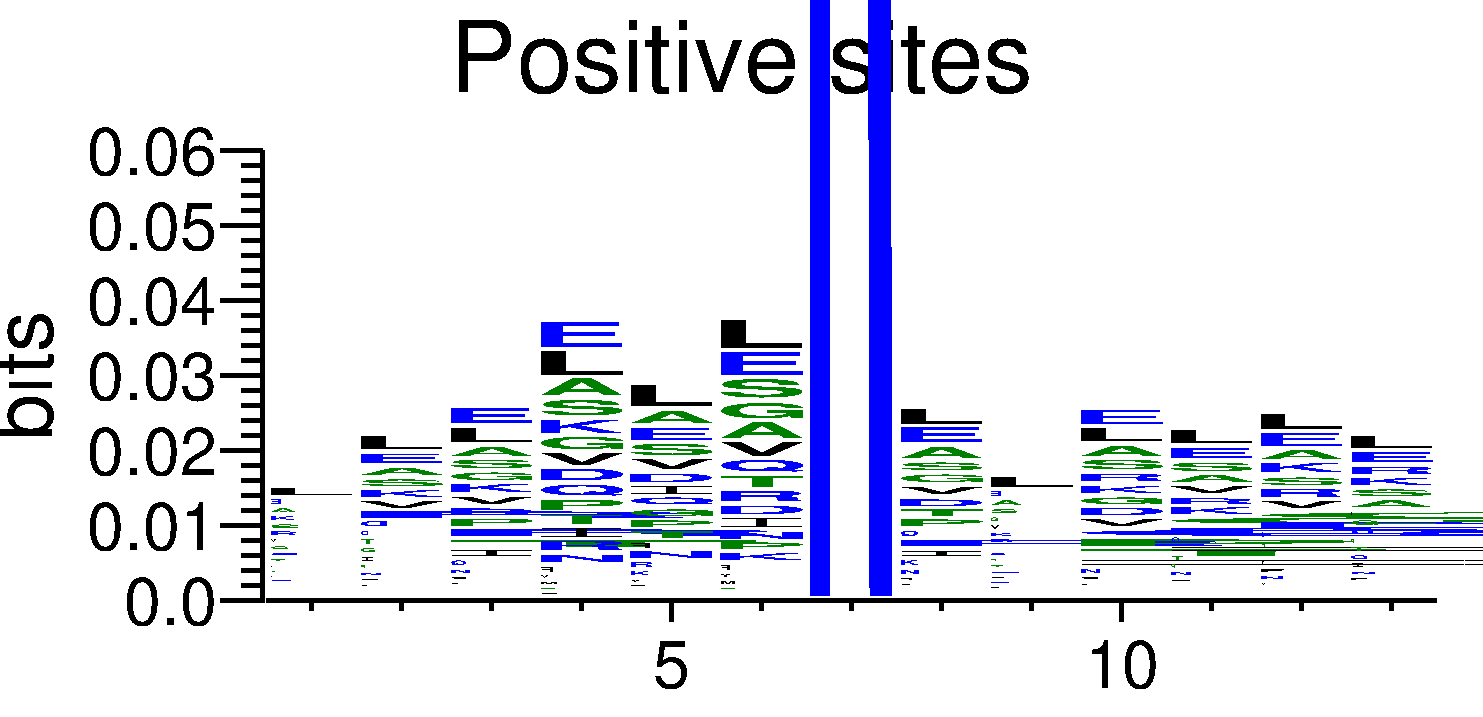
\includegraphics[width=\linewidth]{images/positive_logo_zoom.png}
            \caption{Logo of positive sequences (zoom-in)}
            \label{fig:pos-zoom}
        }
        \hfill
        \parbox{0.5\linewidth}{
            \centering
            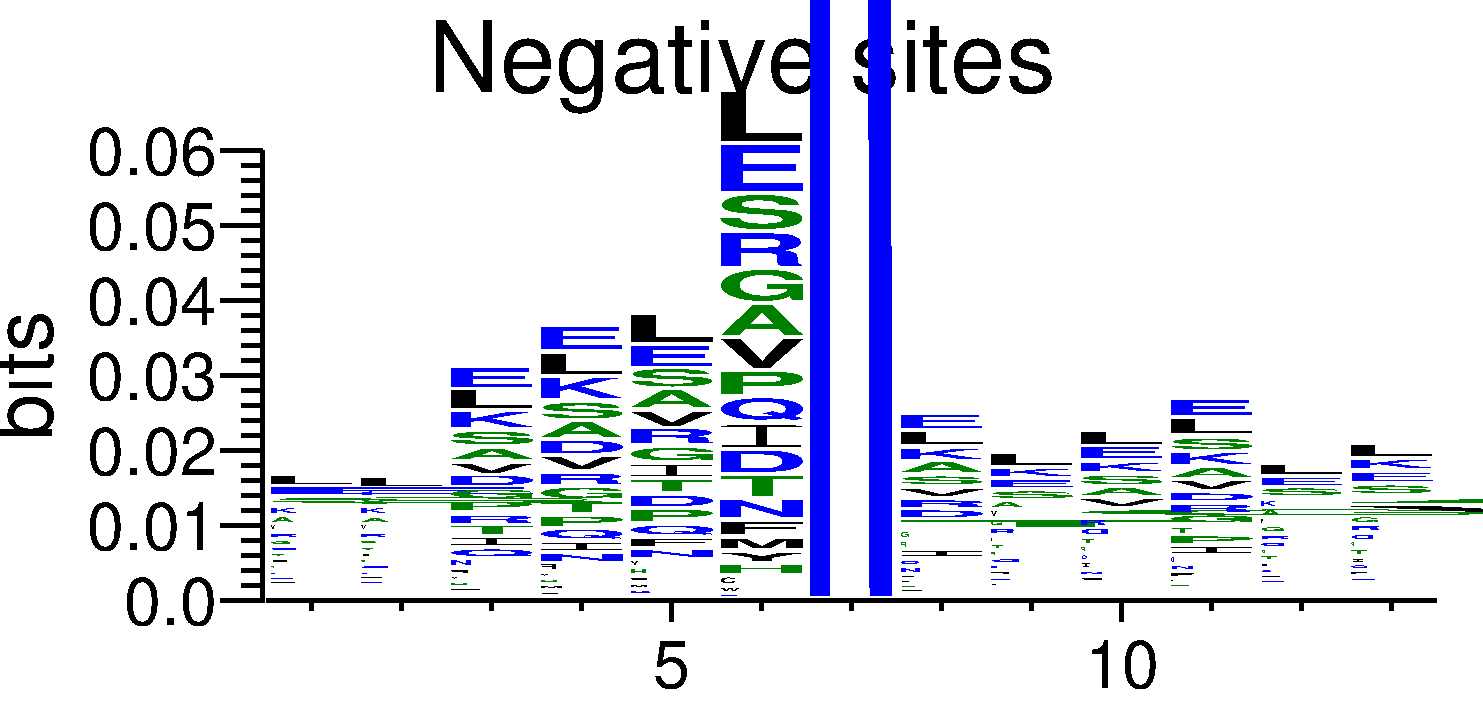
\includegraphics[width=\linewidth]{images/negative_logo_zoom.png}
            \caption{Logo of negative sequences (zoom-in)}
            \label{fig:neg-zoom}
        }
    \end{figure}
    \begin{figure}[htbp]
        \parbox{0.5\linewidth}{
            \centering
            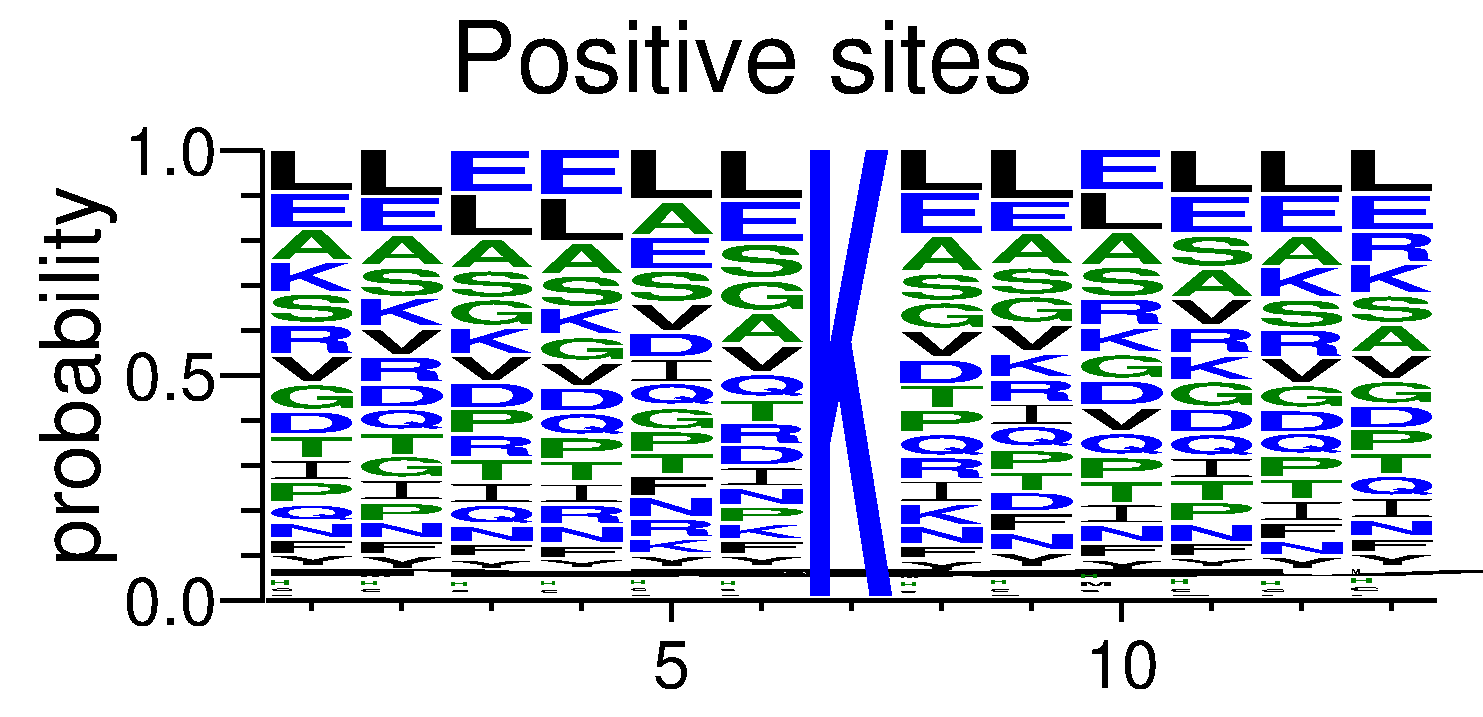
\includegraphics[width=\linewidth]{images/positive_prob.png}
            \caption{Probability plot of positive sequences}
            \label{fig:pos-prob}
        }
        \hfill
        \parbox{0.5\linewidth}{
            \centering
            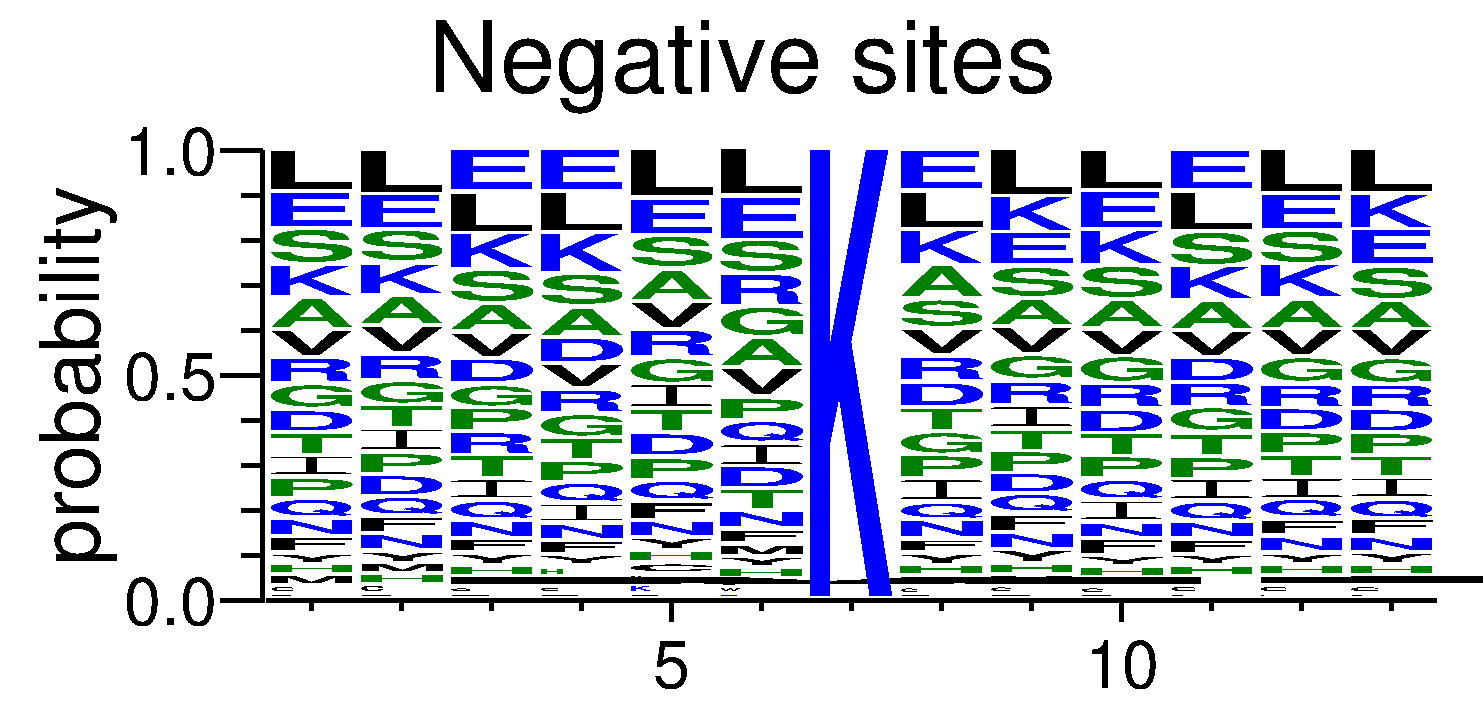
\includegraphics[width=\linewidth]{images/negative_prob.png}
            \caption{Probability plot of negative sequences}
            \label{fig:neg-prob}
        }
    \end{figure}


    \textbf{Two sample logo: }Comparing between 7,429 positive and 32,141 negative sequences, it is realized that Q is frequently enriched in the flanking region of ubiquitination sites. It is also noticable that K is often depleted in the positive samples. The two sample logo plot generated by TwoSampleLogo is shown in Figure~\ref{fig:twosample}

    \begin{figure}[htbp]
        \centering
        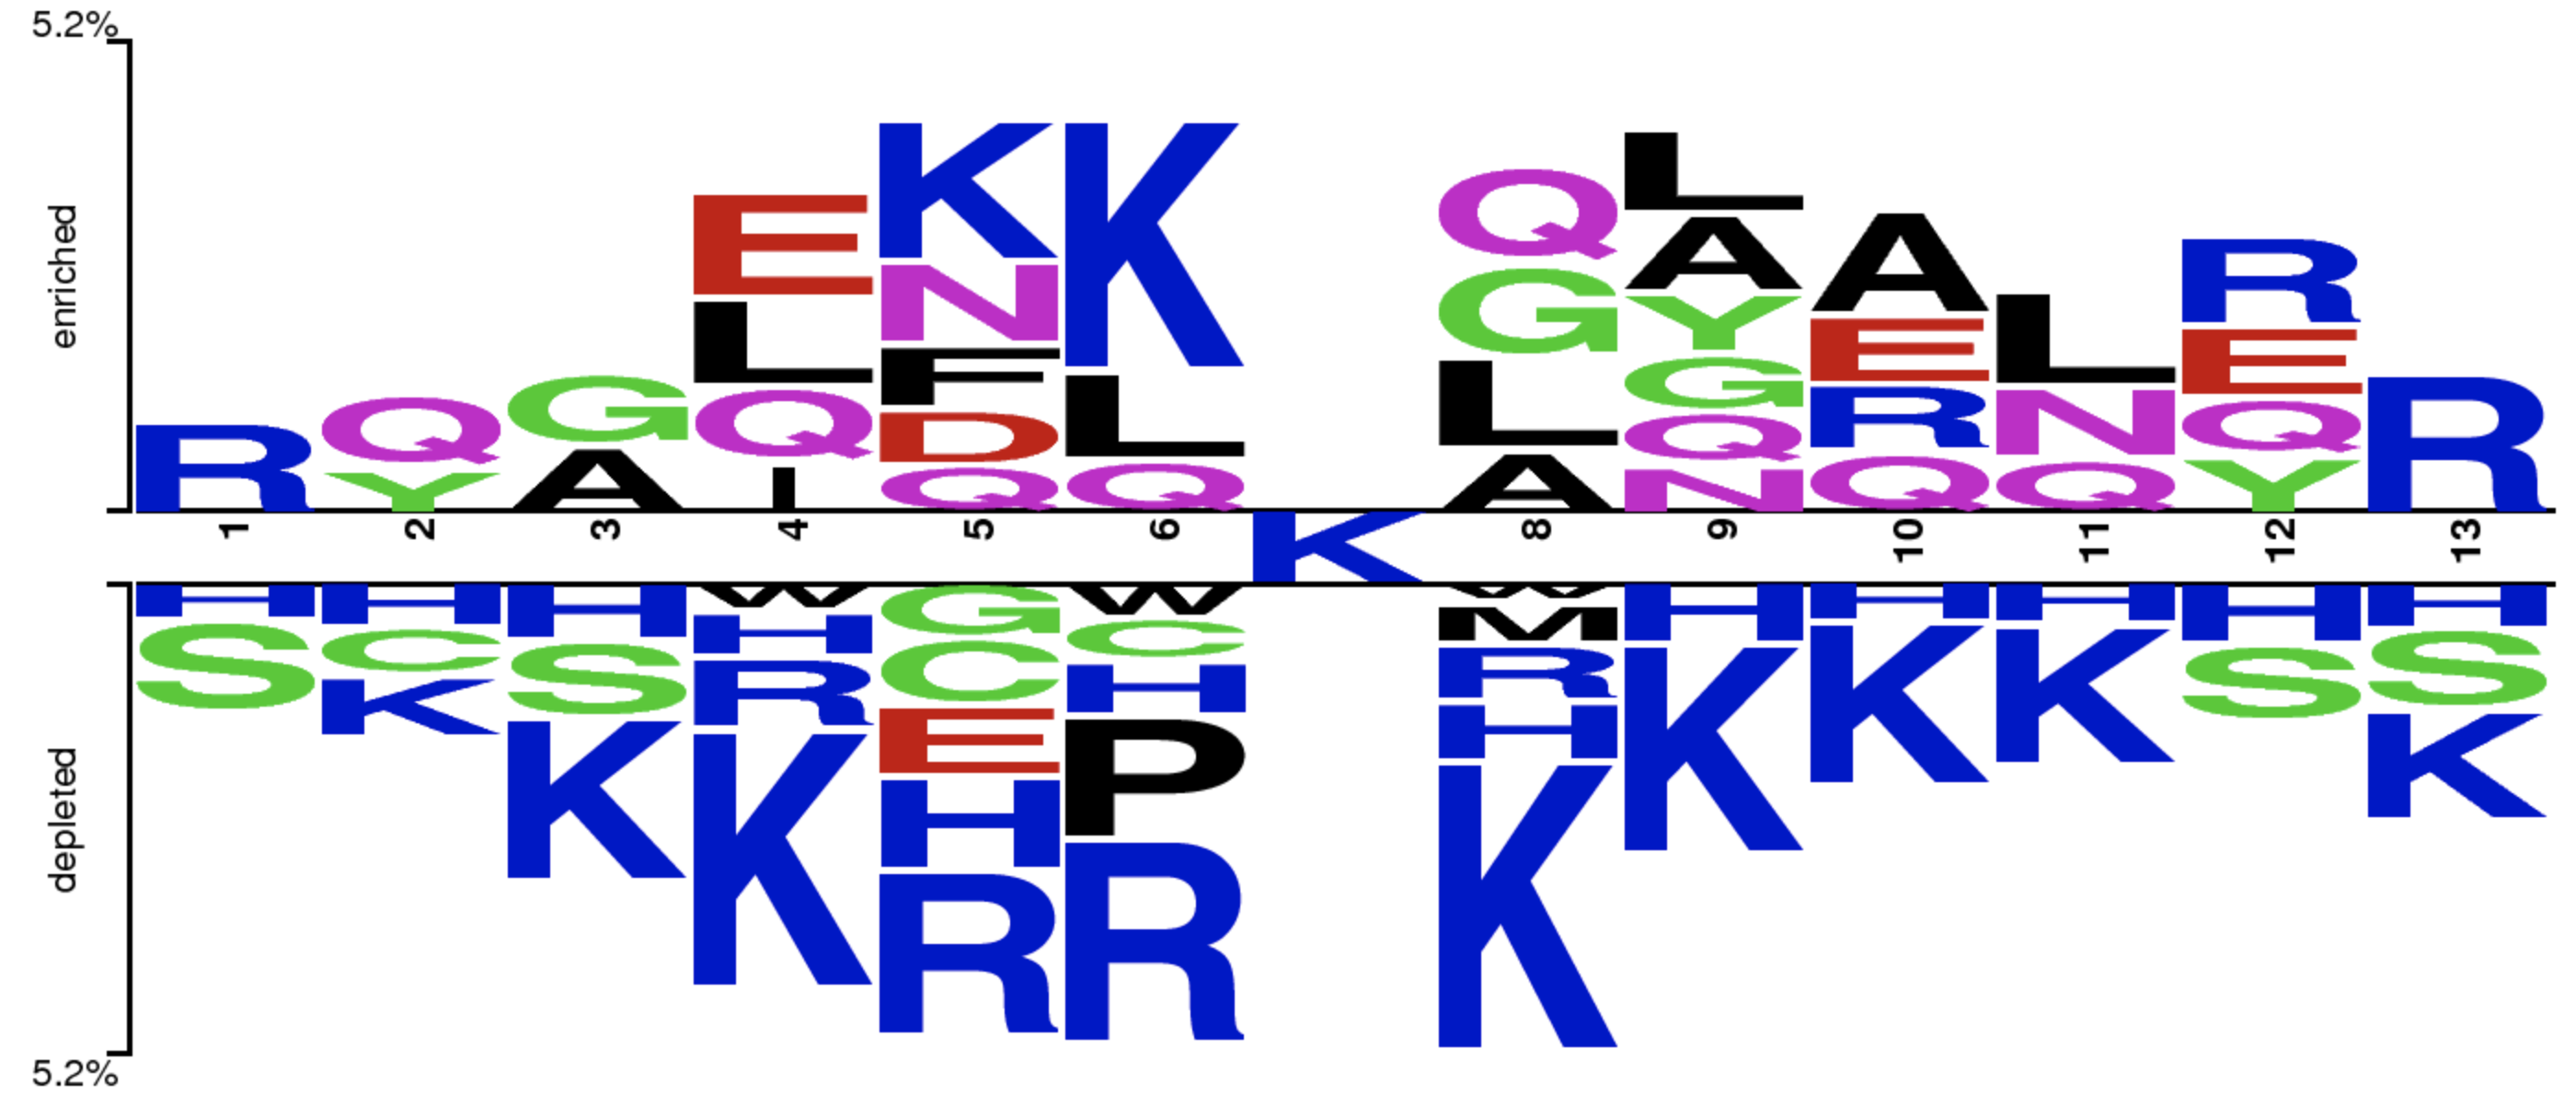
\includegraphics[width=0.8\linewidth]{images/twosamplelogo.png}
        \caption{Two sample logo. This figure is generated by TwoSampleLogo by comparing positive and negative samples. }
        \label{fig:twosample}
    \end{figure}

    \item Finally, Please give out a comparison of AAC (Amino acid composition) between positive and negative sequences in terms of bar-chart visualization. (15 points)
    
    AAC of a sequence is calculated by the following formula:
    $$
    \text{AAC}x=\dfrac{\text{Occurance of amino acid }x}{\text{Length of the sequence}}
    $$
    Using this formula, the average AAC for positive and negative sequences are calculated. Figure~\ref{fig:AAC} shows the comparison between positive and negative samples. It is quite clear that the percentage of K (lysine) is higher in negative sequences than positive ones. This result aligns with the previous Figure~\ref{fig:twosample} that K is frequently depleted in positive sequences. In addition, A (alanine) and Q (glutamine) appears more frequently in positive samples.
    \begin{figure}[t]
        \centering
        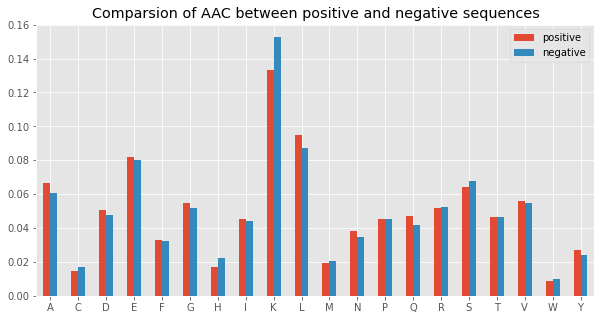
\includegraphics[width=0.8\linewidth]{images/AACcomparison.png}
        \caption{Comparison of AAC}
        \label{fig:AAC}
    \end{figure}
\end{enumerate}
\end{document}